\section{Physical Target Acquisition Study}
To understand the accuracy and performance of head-orientation-based  selection through our device, we carried out a comparative target acquisition study, where participants had to connect to wireless nodes distributed in a room with our technique, and with an alternate list selection approach.

\begin{figure}[t]
\centering
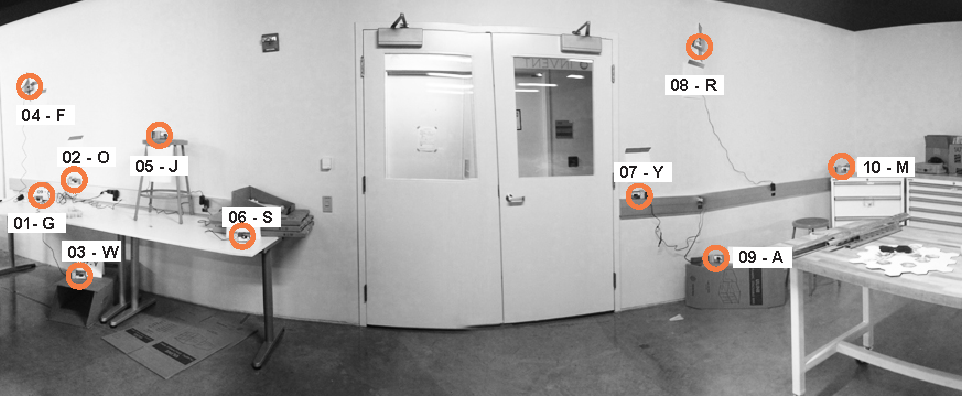
\includegraphics[width=1.0\columnwidth]{figures/targeting-study-layout.pdf}
\caption{In the targeting study, participants had to find and select one of 10 targets in a lab environment. Targets were called out by number; for the list mode condition, participants need to match numbers to letters.}
\label{fig:targeting-study-layout}
\end{figure}

\subsection{Apparatus}
In an indoor environment, 10 wireless nodes are spread across a room at various heights and distances (Figure~\ref{fig:targeting-study-layout}). The nodes are stand-ins for potential smart appliances and have all relevant functionality for targeting and wireless communication, but do not control any actual appliances. Each node is an embedded wireless system with a microcontroller, IR receiver, a wireless XBee radio, and three status LEDs (Figure~\ref{fig:target}). An yellow LED indicates that the device is the target that should be selected in the current trial; a red LED lights up whenever the device receives an IR signal from Glass; a blue LED shows when participants have successfully connected to a device, and is also used for disambiguation when multiple targets are within IR range. Next to each target, a paper sheet shows a number and letter combination, which is used for uniquely identifying the device. The numbers are the primary identifiers, ordered from left to right in the room. This ordering makes it easy to locate them, which simulates looking towards an appliance with a well-known location in a room, and minimizes visual search time.

\begin{figure}[b]
\centering
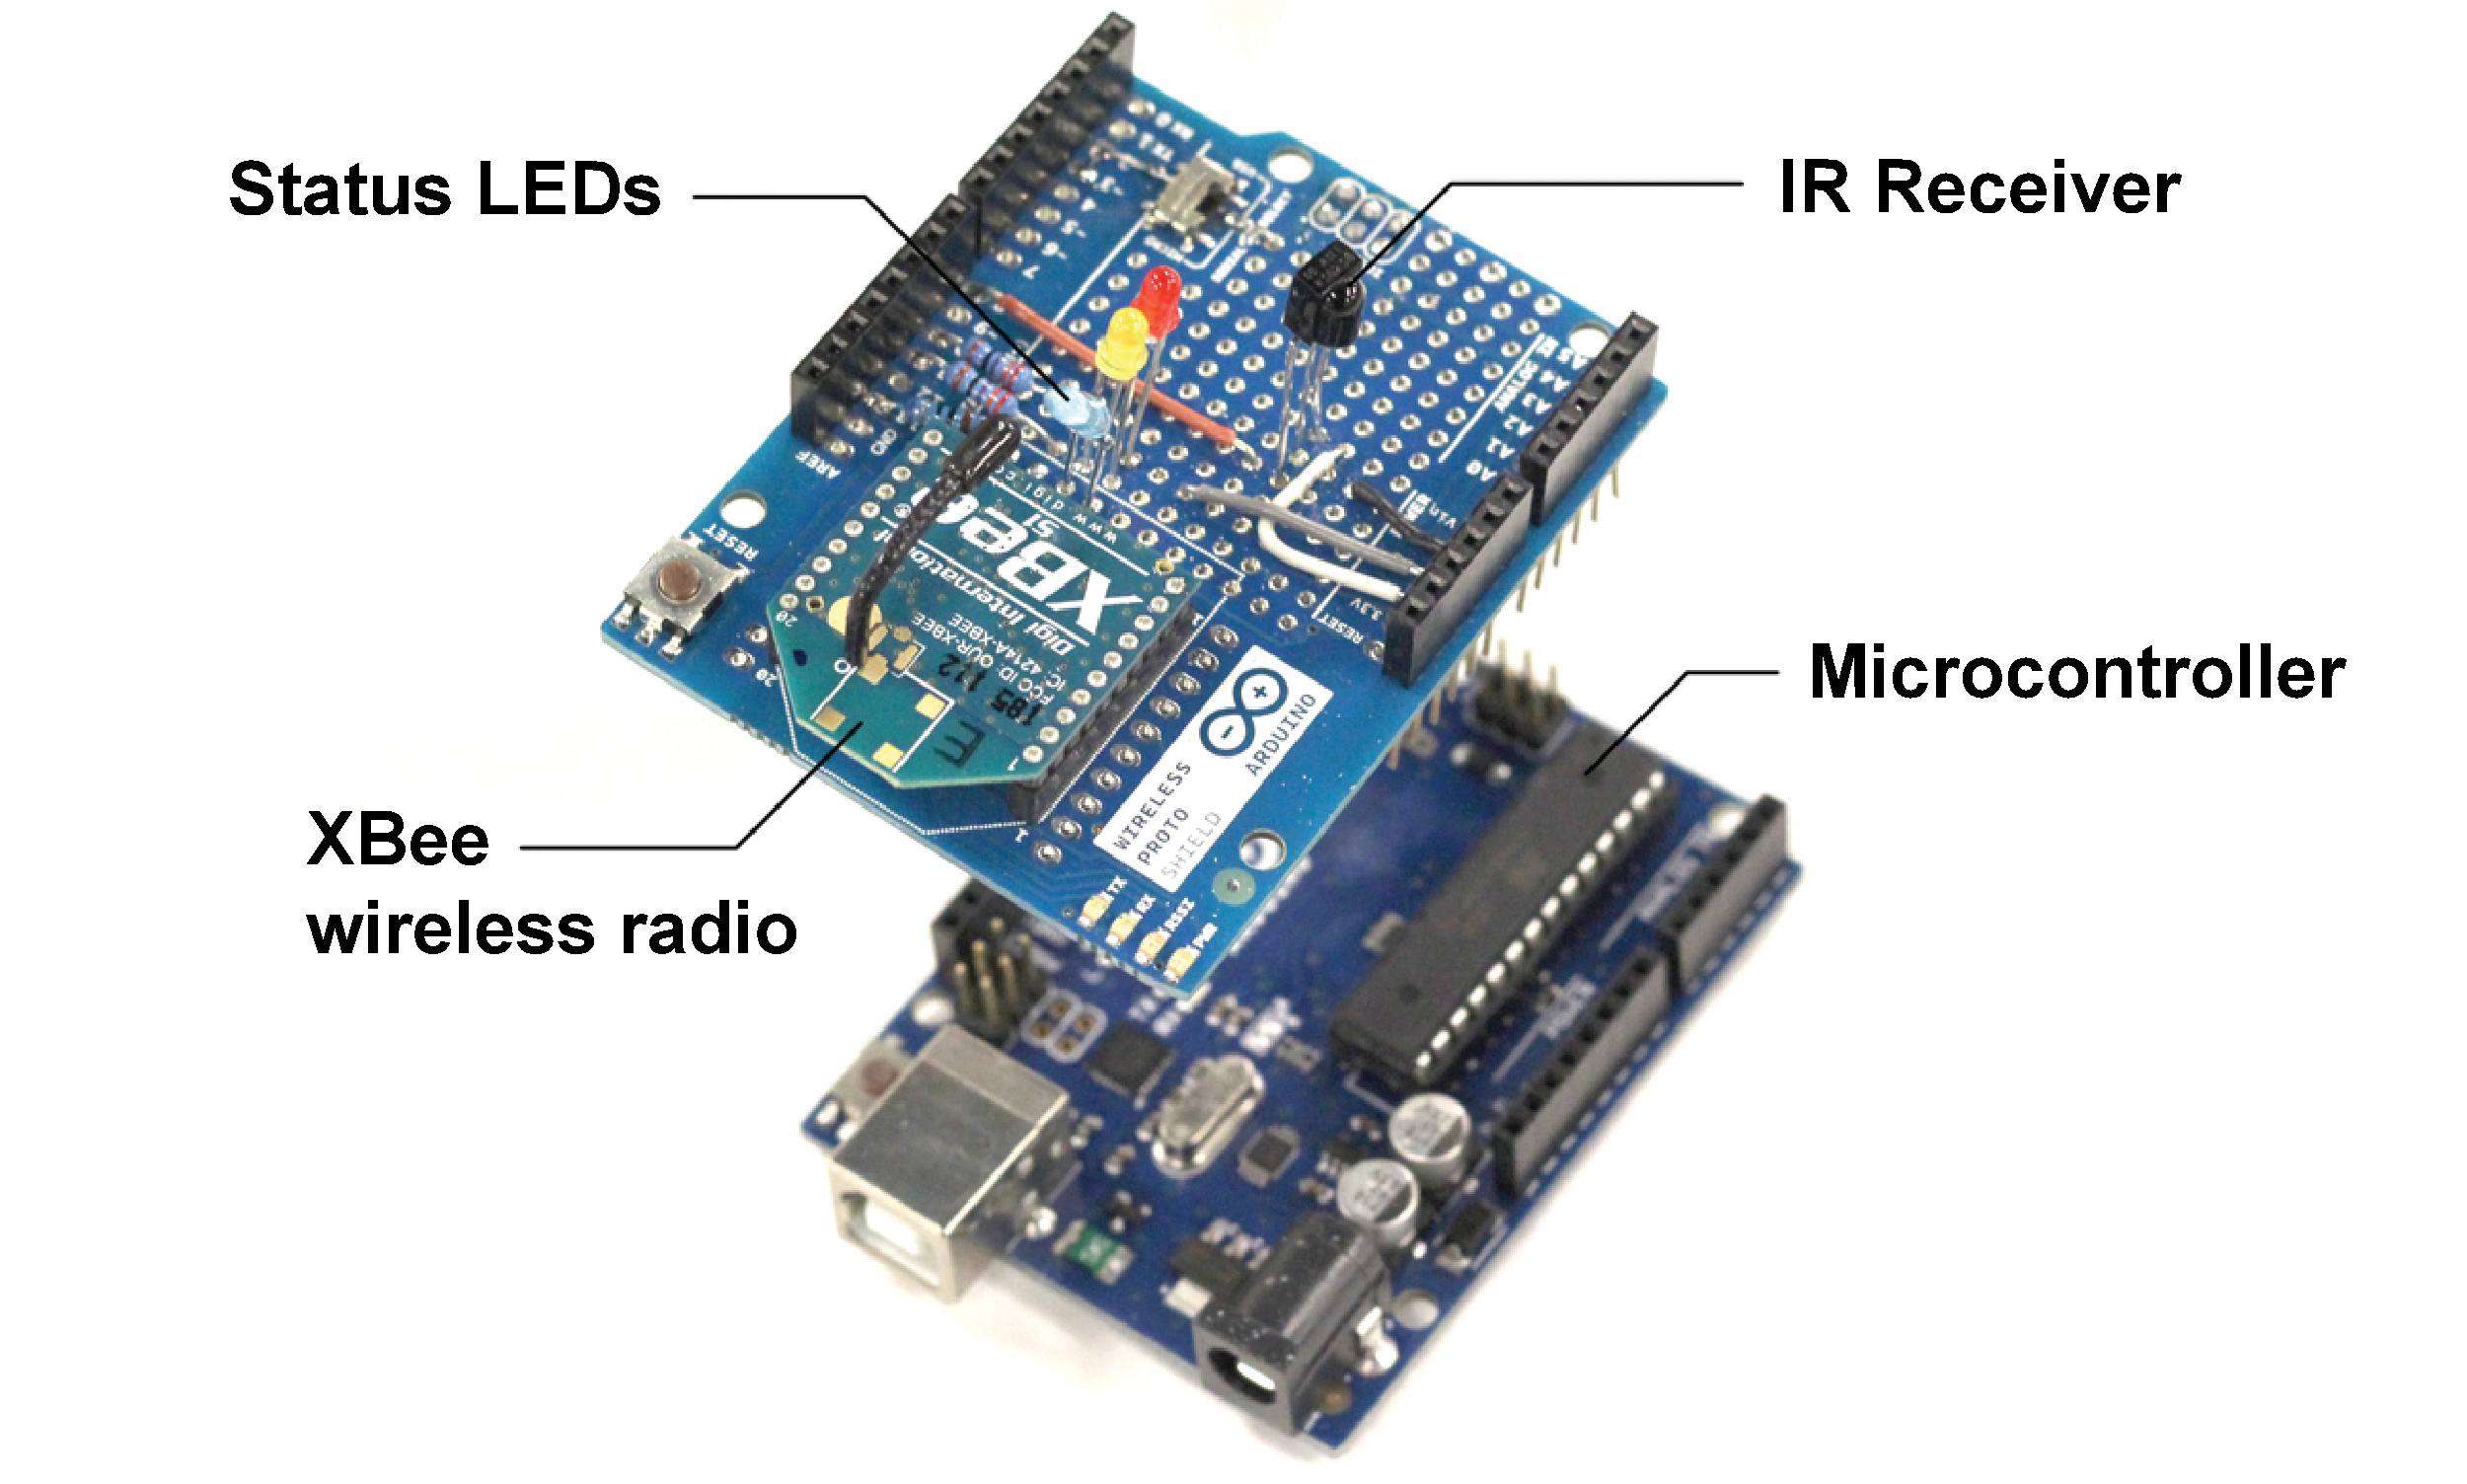
\includegraphics[width=0.8\columnwidth]{figures/study-node.pdf}
\caption{An example node from the targeting study --- we constructed 10 such nodes - each mounted in a box.}
\label{fig:target}
\end{figure}

\subsection{Methodology}
In our within-subjects design, participants performed 15 target acquisition tasks each with two interaction styles. In the {\em infrared} mode condition, participants used our IR targeting approach; in the {\em list} mode condition, participants had to look up a device's letter code on the printed paper next to the device and then select that letter code from a list displayed on their Glass device. The list was navigated with swipe motions on the Glass touchpad. For each task, participants started at a fixed position in the room. The experimenter called out a number and simultaneously started a timer. Participants then had to find the corresponding device (by looking for its printed code). In the {\em infrared} mode, participants then selected and acquired the target by aiming the IR beam at the target, and confirmed their selection with a touch pad tap. If more than one target was within range, participants had to either use the disambiguation dialog or reposition themselves. In the {\em list} mode, participants had to read the letter next to the number and then select that letter by browsing a linear list shown in their Glass display. While the list was alphabetized, letter arrangement in the room was not. This design required participants to find the target in the room before starting a list navigation to keep visual search times similar in each condition.

Afterwards, participants completed a survey that elicited answers to Likert-scale questions as well as open-ended answers about their experience.

\subsection{Participants}
We recruited 14 participants from our institution. 13 had never used Glass before. 4 wore prescription glasses, which may have affected their task performance as wearing glasses beneath Glass makes it more cumbersome to secure the position of Glass and to adjust the screen to the optimal angle. Half of them performed {\em infrared} mode first and the other half did {\em list} mode first.

\subsection{Measures}
The main measures were {\bf target acquisition time}: the time required to identify, select, and connect to a wireless target device; and {\bf user preference}: which interface users preferred for the task after completing the study.

\subsection{Results}
\subsubsection{Performance data}
The time to complete each task can be broken down into the following pieces:

$t_{infrared}=t_{locate}[+t_{reorient}][+t_{disambiguate}]+t_{tap}$

$t_{list}=t_{locate}+t_{listnav}+t_{tap}$

In both conditions, participants first have to locate the target announced by the experimenter through visual search ($t_{locate}$). In the {\em infrared} mode, participants may then directly confirm their selection if only a single target was selected ($t_{tap}$). However, if they don't immediately receive feedback that their target was selected, or if multiple targets were selected, users either have change their position or head orientation ($t_{reorient}$) or they have to step through the on-screen disambiguation dialog ($t_{disambiguate}$). In the {\em list} mode, participants must scroll through the list to find the desired target identifier ($t_{listnav}$).
Thus, {\em infrared} will show a performance benefit if $(t_{reorient}+t_{disambiguate})<t_{listnav}$. This depends on the number of total devices in the environment (increasing $t_{listnav}$), and their density (which will increase $t_{disambiguate}$). 

\begin{figure}[t]
\centering
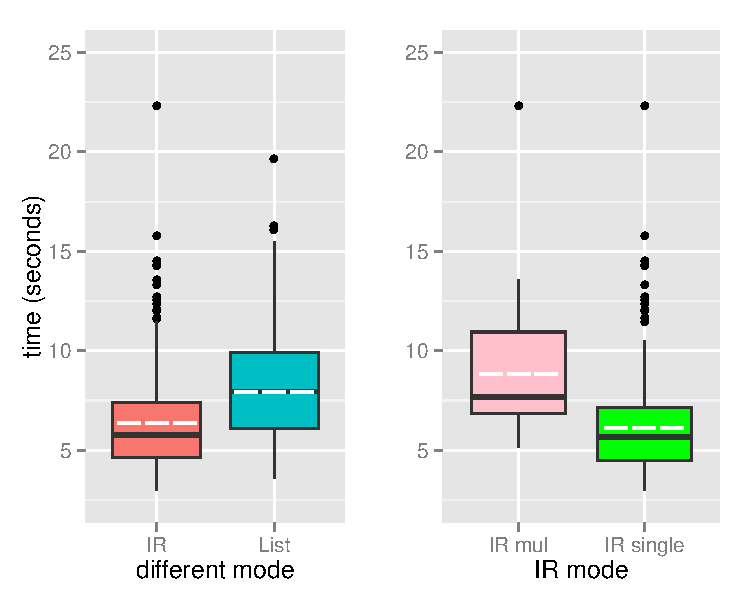
\includegraphics[width=1.0\columnwidth]{figures/R_time_by_Category.pdf}
\caption{Boxplot of task completion times for the comparison between {\em infrared} mode and {\em list} mode (A), between IR multiple responses cases and IR single response cases (B). The centers of boxes are median values, while white dashed lines are mean values; they are also annotated on the top part.}
\label{fig:selection-times}
\end{figure}

We first show results for 10 targets and then discuss extrapolations of these results. Average target acquisition time $t_{infrared}$ was 6.67 seconds, while $t_{list}$ was 8.86 seconds (Figure~\ref{fig:selection-times}A). This difference is significant (Student's t-test, $t(279)=-3.81, p=0.00017$). % \bjoern{you need to report the t statistic and degrees of freedom as well - t(df)= n,p=m.} 

To further understand the performance gain in {\em infrared} mode, especially the factor $t_{disambiguate}$, we compare selection times when multiple devices are targeted (and disambiguation is required) to single-device selection times (Figure~\ref{fig:selection-times}B). When there is a single device, $t_{disambiguate}$ is 0 and it takes 6.40 seconds (on average) to complete the connection. When multiple devices are in range, the time increases to 9.16 seconds, indicating 2.76 seconds required to disambiguate. Though it takes significantly longer ($t(19)=-2.7827, p=0.012$ using t-test) in the {\em multiple} case, these cases made up only 10\% of total infrared trials.
%, even we intentionally placed a few devices nearer to each other. % 19 / (19+168 )

\begin{figure}[t]
\centering
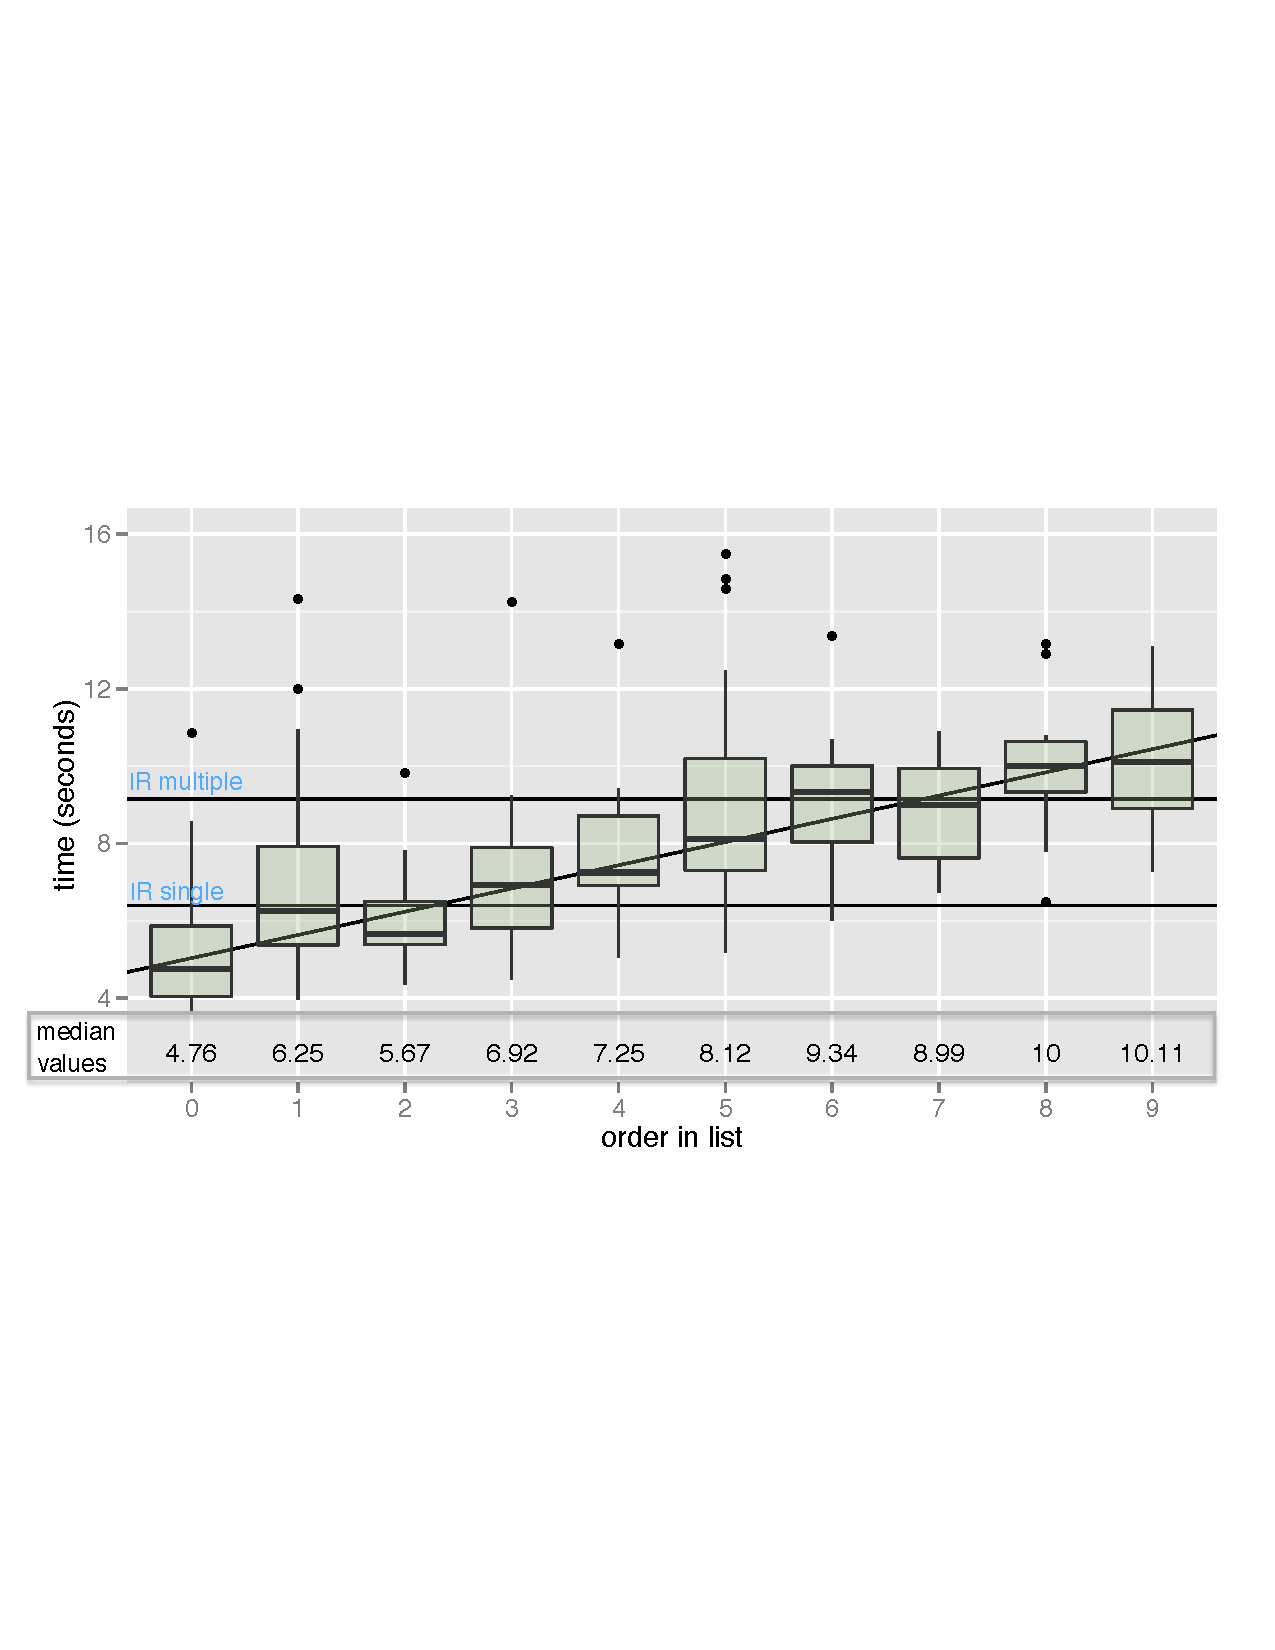
\includegraphics[width=1.0\columnwidth]{figures/R_List_by_Target.pdf}
\caption{Times taken to select a device vs.~the order in the list. The dotted line is a linear fit between the mean times and device orders. Two horizontal lines of mean target acquisition times in {\em infrared} mode are also annotated for comparison.}
 % \bjoern{Add horizontal lines at $t_{IRsingle}$ and $t_{IRmultiple}$.}
\label{fig:time-vs-list-order}
\end{figure}

For each device, $t_{listnav}$ depends on their relative position in the list. Figure~\ref{fig:time-vs-list-order} shows the time it takes to select a device (means and standard deviations) as a function of its list position - the trend line (dotted) enables extrapolation to estimate at what number of devices the {\em infrared} mode interaction techniques will outperform {\em list} mode\footnote{The higher mean value at $order=1$ is caused by one outlier when the participant failed multiple times to connect to the right target}. From the figure, we can see that once the target's order has increased to be larger than 6, the average $t_{listnav}$ would be larger than $t_{reorient} + t_{disambiguate}$. 

% \bjoern{A linear trend is visible, and the regression returns with coefficient of determination ($R^2=0.032$). --- This R value is basically no correlation at all! try to run a correlation only on the median times. }

Participants' selection errors do occur in both conditions. However, error rates were low (1.1\% in {\em infrared} mode, and 2.9\% in {\em list} mode, repspectively). This precludes us from running a more detailed analysis. 

\begin{figure}[t]
\centering
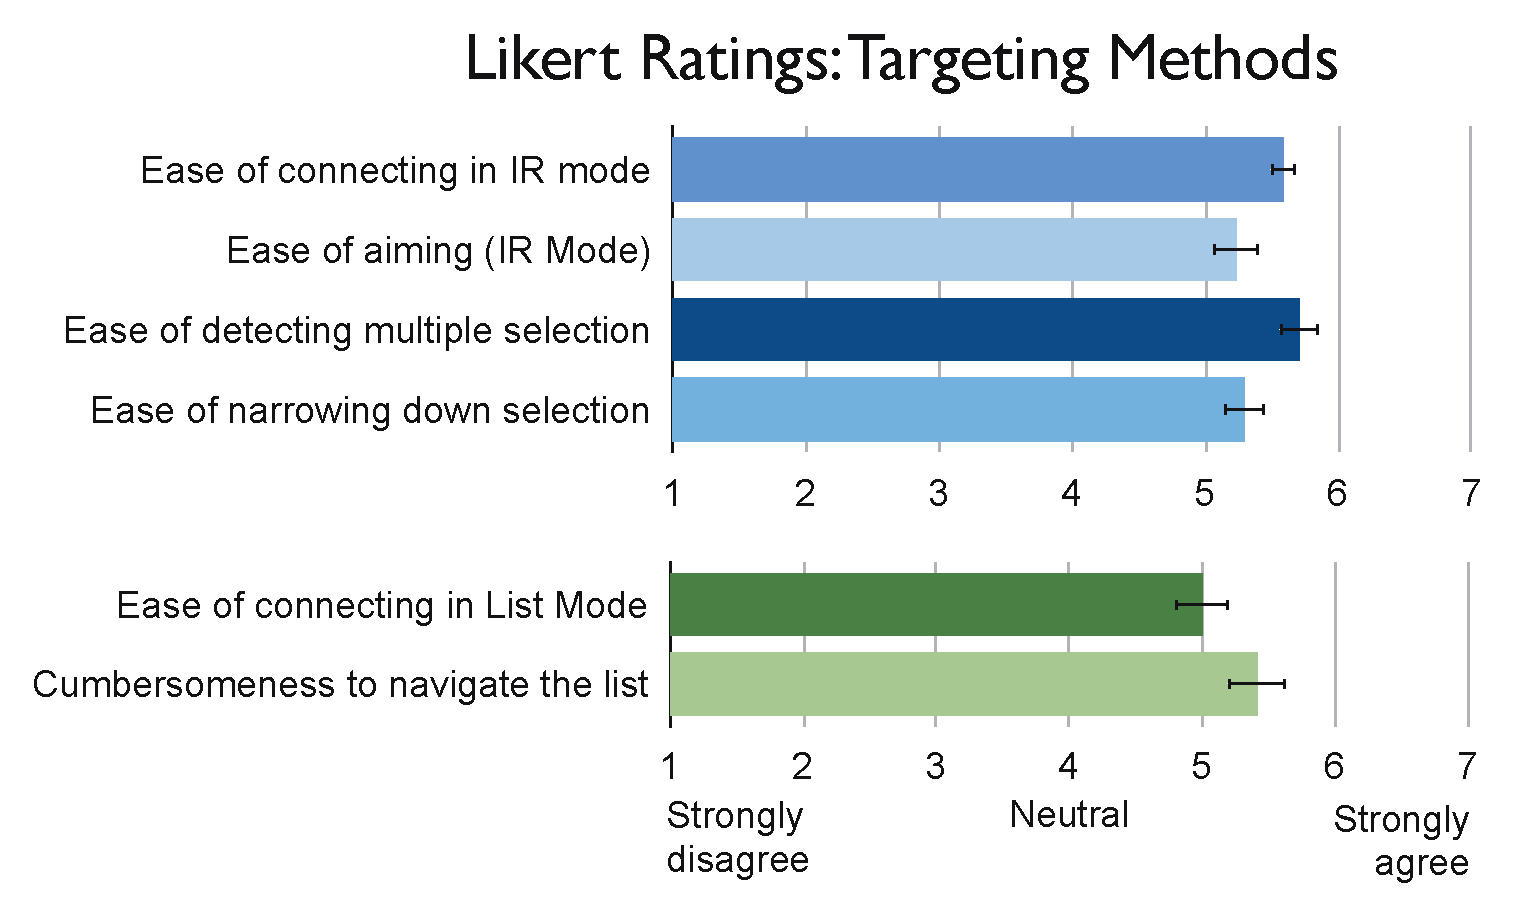
\includegraphics[width=1.0\columnwidth]{figures/target-likert.pdf}
\caption{Likert scale ratings for ease of use of aspects of the targeting task. Error bars show standard error. }
\label{fig:target-likert}
\end{figure}

\subsubsection{Preference}

Eleven of 14 users preferred infrared mode over list mode (three preferred list, one was undecided). While both interfaces were judged similarly on overall ease of connecting, list navigation was also perceived to be cumbersome (see Figure~\ref{fig:target-likert}). As self-report data can easily skew positive as participants try to please experimenters, we also asked participants to elucidate why they preferred one interface over the other.

List mode had certain advantages: It was judged to be more accurate and predictable as there was always exactly one device selected in the list (\studyquote{With the list you never have to worry about accidentally picking up two targets}). Also, it did not require a clear line of sight to the target device so participants did not have to move from their starting position (\studyquote{The shortcoming of the IR mode was that you had to be a certain distance away in order for it to detect the appliance}). 

On the other hand, list mode was judged to be more \studyquote{annoying} and tedious. The temple-based touchpad for selection was difficult to use for a participant with long hair: \studyquote{List mode was physically difficult for me to navigate, since my long hair wasn't tied back and it kept interfering with my swiping.} Another participant also commented on the ergonomic challenge of touchpad use on Glass: \studyquote{The strength of the IR mode was that I didn't have to use my fingers as much to control. If the items were spaced relatively far apart, it was easy to select a specific appliance.}

One noted benefit of infrared mode was a feeling that it was \studyquote{more direct [than list mode]}, allowing users to focus on the targeted objects instead of the screen. One subject called it \studyquote{natural to interact with things just by looking at them}. Another mentioned that \studyquote{it's really convenient that what I'm looking at is what I'm targeting}. 

A few perceived weaknesses of IR mode were the necessity to move the head in order to control a device and the imperfect mapping of gaze to target. One participant said that it was \studyquote{awkward to be aiming your head at things, tweaking back and forth to get it right}. Another noted that observing the head movement didn't capture the site of her attention, because \studyquote {eye movement is an important part of how people look around}. Users had to learn the usable angle of the IR emitter before they became successful at controlling the devices: \studyquote{I had to compensate by tilting my head up a little bit.}



%IR mode has semantic meaning (like I said).  I'm likely to want visual feedback from any distant device I'm trying to control, and since I'm already looking at it, this is very easy to get.  List mode was physically difficult for me to navigate, since my long hair wasn't tied back and it kept interfering with my swiping.  Another comment about list mode was that swiping faster didn't seem to navigate the list faster, which would have been convenient for accessing items like W and Y very far from the beginning of the list.  This could also be partially overcome by using a circular linked list (where the list wraps from Y to A) instead of a one-way list.
%With the list you never have to worry about accidentally picking up two targets, but since you always have to swipe through a (longer) list that's not much of an advantage.
%List mode felt like I could be more confident in what client I was choosing because I couldn't select more than one client. The IR mode was a little more natural because it involved less clicking and navigating, but it felt easier to select the wrong client which made the list mode more comfortable. 
%"The shortcoming of the List mode was that the list didn't wrap around. So for example if I wanted to go to Y, I couldn't just go left from A—I had to scroll through all the letters in between.

%The strength of the list mode was that it's pretty accurate, so as long as I swiped the correct amount, I could activate and power off the appliances. I also didn't have to move at all, although perhaps that is a shortcoming because otherwise we might just all turn into Wall-E people.

%The strength of the IR mode was that I didn't have to use my fingers as much to control. If the items were spaced relatively far apart, it was easy to select a specific appliance. 

%The shortcoming of the IR mode was that you had to be a certain distance away in order for it to detect the appliance. "
%The List Mode is easier to choose the desired item when the item list is short. It became a bit frustrated when I had to swipe many times in order to get to the targeted item. The IR mode works more intuitive in this case, but need a longer time to learn and get used to it.
%list mode is easier to select what you want, but may take a while to get to since you can only swipe through one at a time; IR is quicker and more intuitive, but unstable
%"list mode is annoying. i find myself counting how many swipes i have to do.

%IR mode is fun and pretty convenient"


